\appendix
\chapter{List of abbreviations}
\begin{itemize}
\item \textbf{AM}: \textbf{A}mplitude \textbf{M}odulated
\item \textbf{AGN}: \textbf{A}ctive \textbf{G}alactic \textbf{N}ucleus
\item \textbf{CMB}: \textbf{C}osmic \textbf{M}icrowave \textbf{B}ackground
\item \textbf{CP}: \textbf{C}harge \textbf{P}arity
\item \textbf{DAQ}: \textbf{D}ata \textbf{AQ}uisition system
\item \textbf{DnR}: \textbf{D}irect a\textbf{N}d \textbf{R}efracted
\item \textbf{DSNB}: \textbf{D}iffuse \textbf{S}upernova \textbf{N}eutrino \textbf{B}ackground
\item \textbf{FFT}: \textbf{F}ast \textbf{F}ourrier \textbf{T}ransform
\item \textbf{GRBs}: \textbf{G}amma-\textbf{R}ay \textbf{B}ursts
\item \textbf{MSW}: \textbf{M}ikheyev–\textbf{S}mirnov–\textbf{W}olfenstein
\item \textbf{PMNS}: \textbf{P}ontecorvo-\textbf{M}aki-\textbf{N}akagawa-\textbf{S}akata
\item \textbf{RADIANT}: \textbf{RA}dio \textbf{DI}gitizer and \textbf{A}uxiliary \textbf{N}eutrino \textbf{T}rigger
\item \textbf{RNO-G}: \textbf{R}adio \textbf{N}eutrino \textbf{O}bservatory in \textbf{G}reenland
\item \textbf{RF}: \textbf{R}adio \textbf{F}requency
\item \textbf{SNEWS}: \textbf{S}uper\textbf{N}ova \textbf{E}arly \textbf{W}arning \textbf{S}ystem
\item \textbf{UHE}: \textbf{U}ltra \textbf{H}igh \textbf{E}nergy 
\item \textbf{UHECRs}: \textbf{U}ltra \textbf{H}igh \textbf{E}nergy \textbf{C}osmic \textbf{R}ay\textbf{s}
\end{itemize}
\chapter{Extra Figures}
\label{app:ExtraFigures}
\begin{figure}[h]
	\centering
	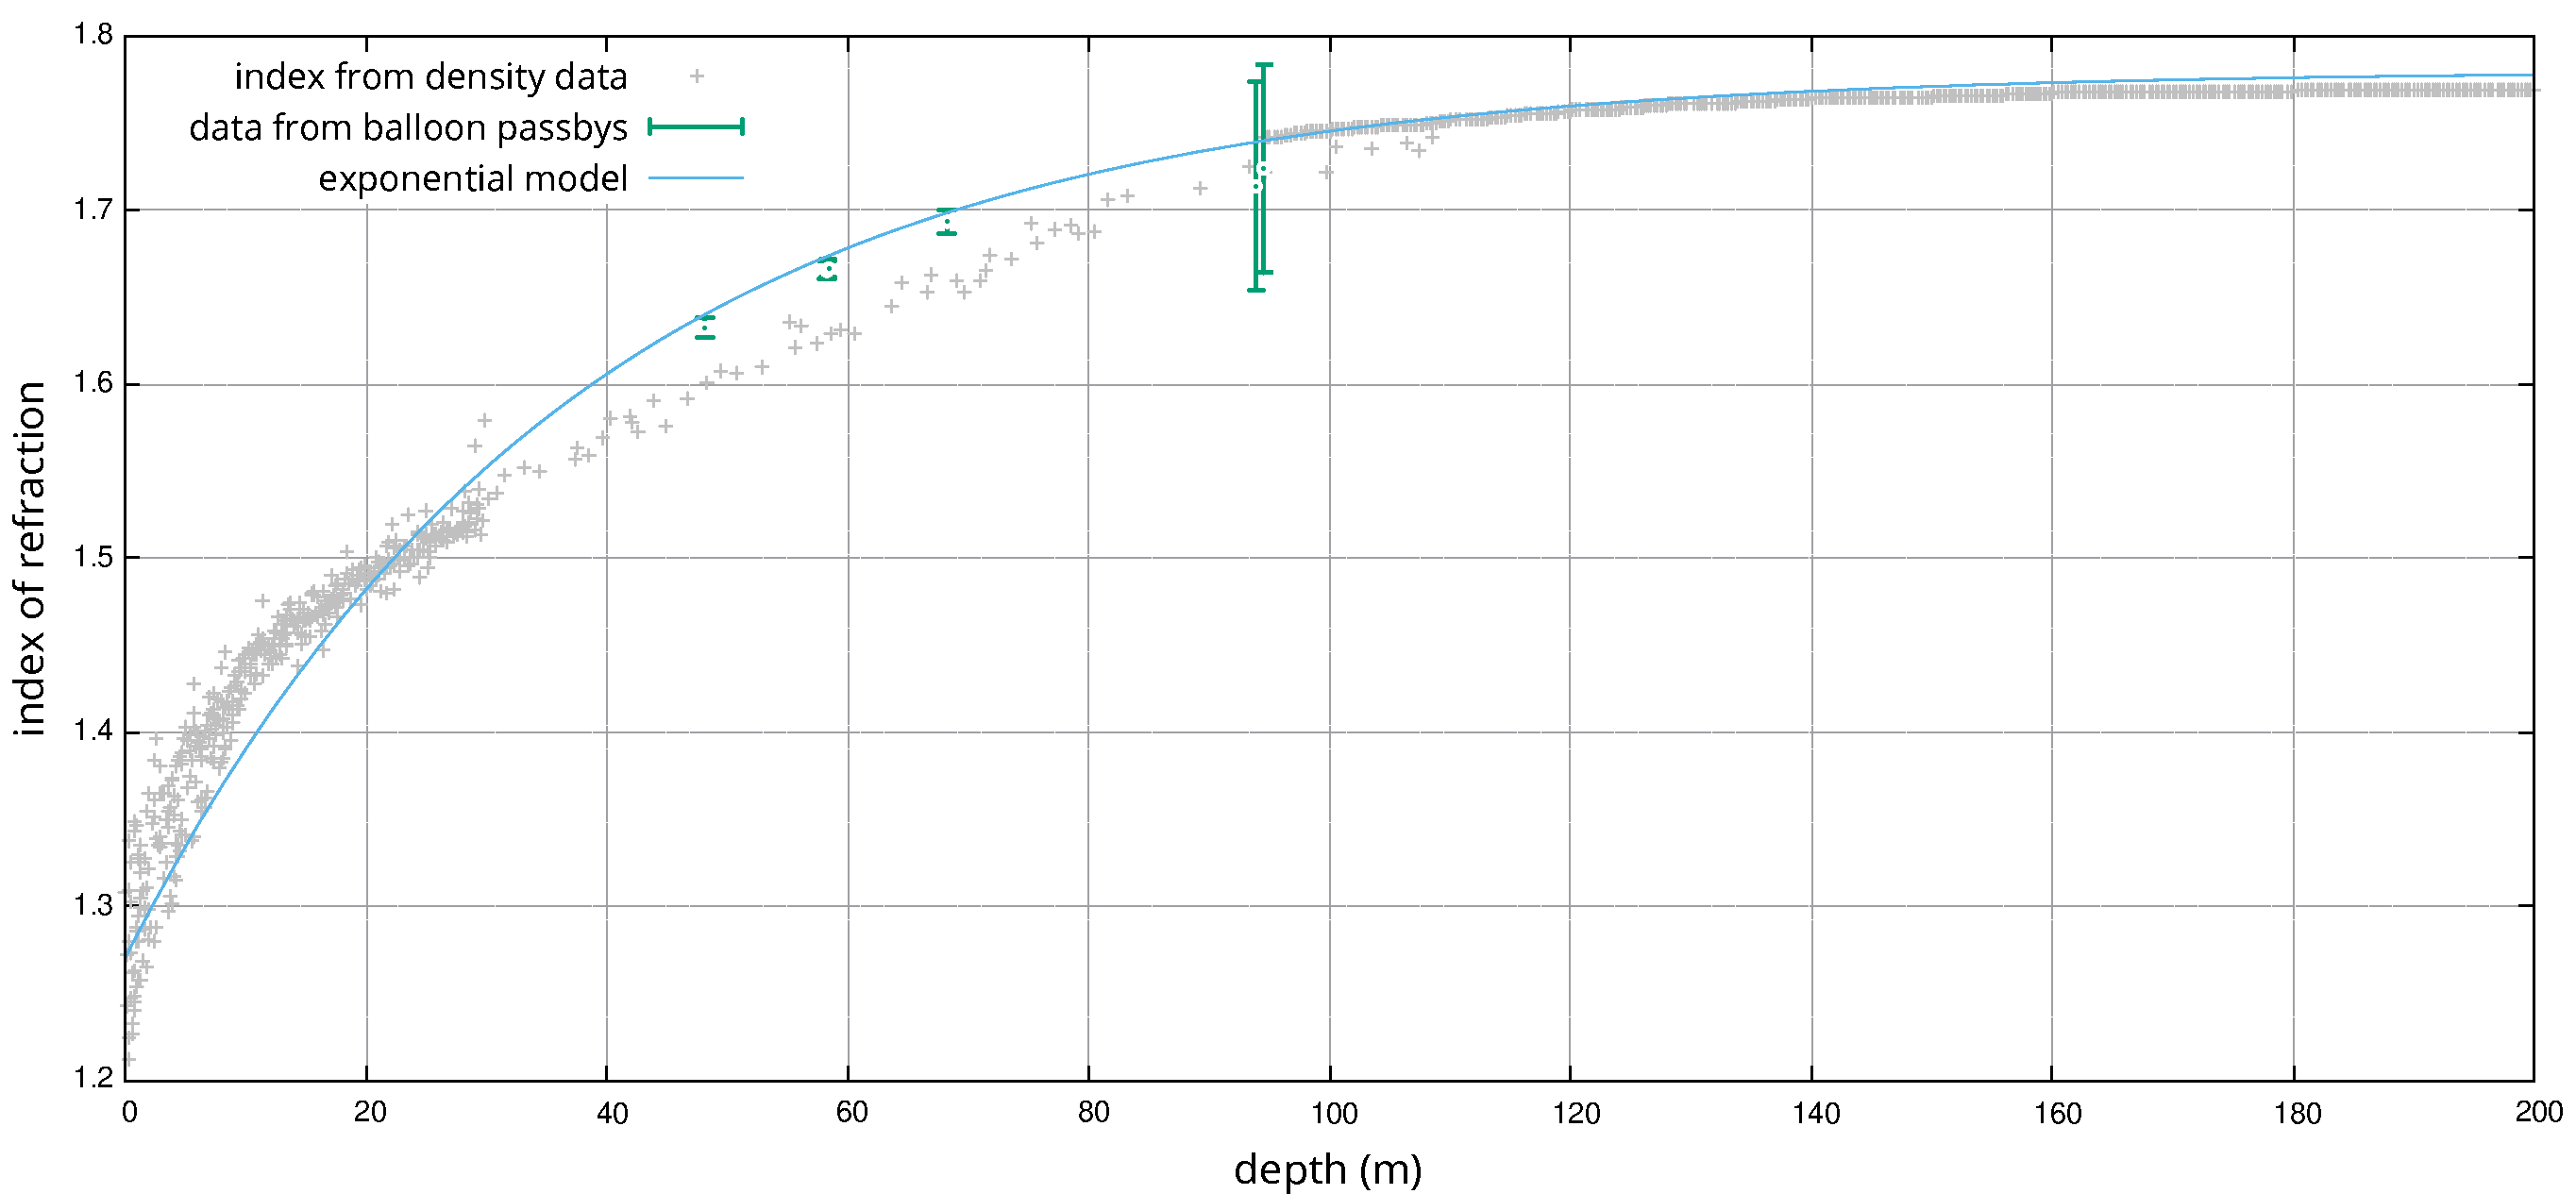
\includegraphics[width=\textwidth]{figures/ResultsOtherLinear.pdf}
  \caption{Changing the linear index-density relation from $n(z) = 1+0.78\rho(z)$ to $n(z) = 1+0.77\rho(z)$ (shown here) seems
to make our phased array measurements lie closer to the density data.}
	\label{fig:ResultsOtherLinear}
\end{figure}
\begin{figure}
	\centering
	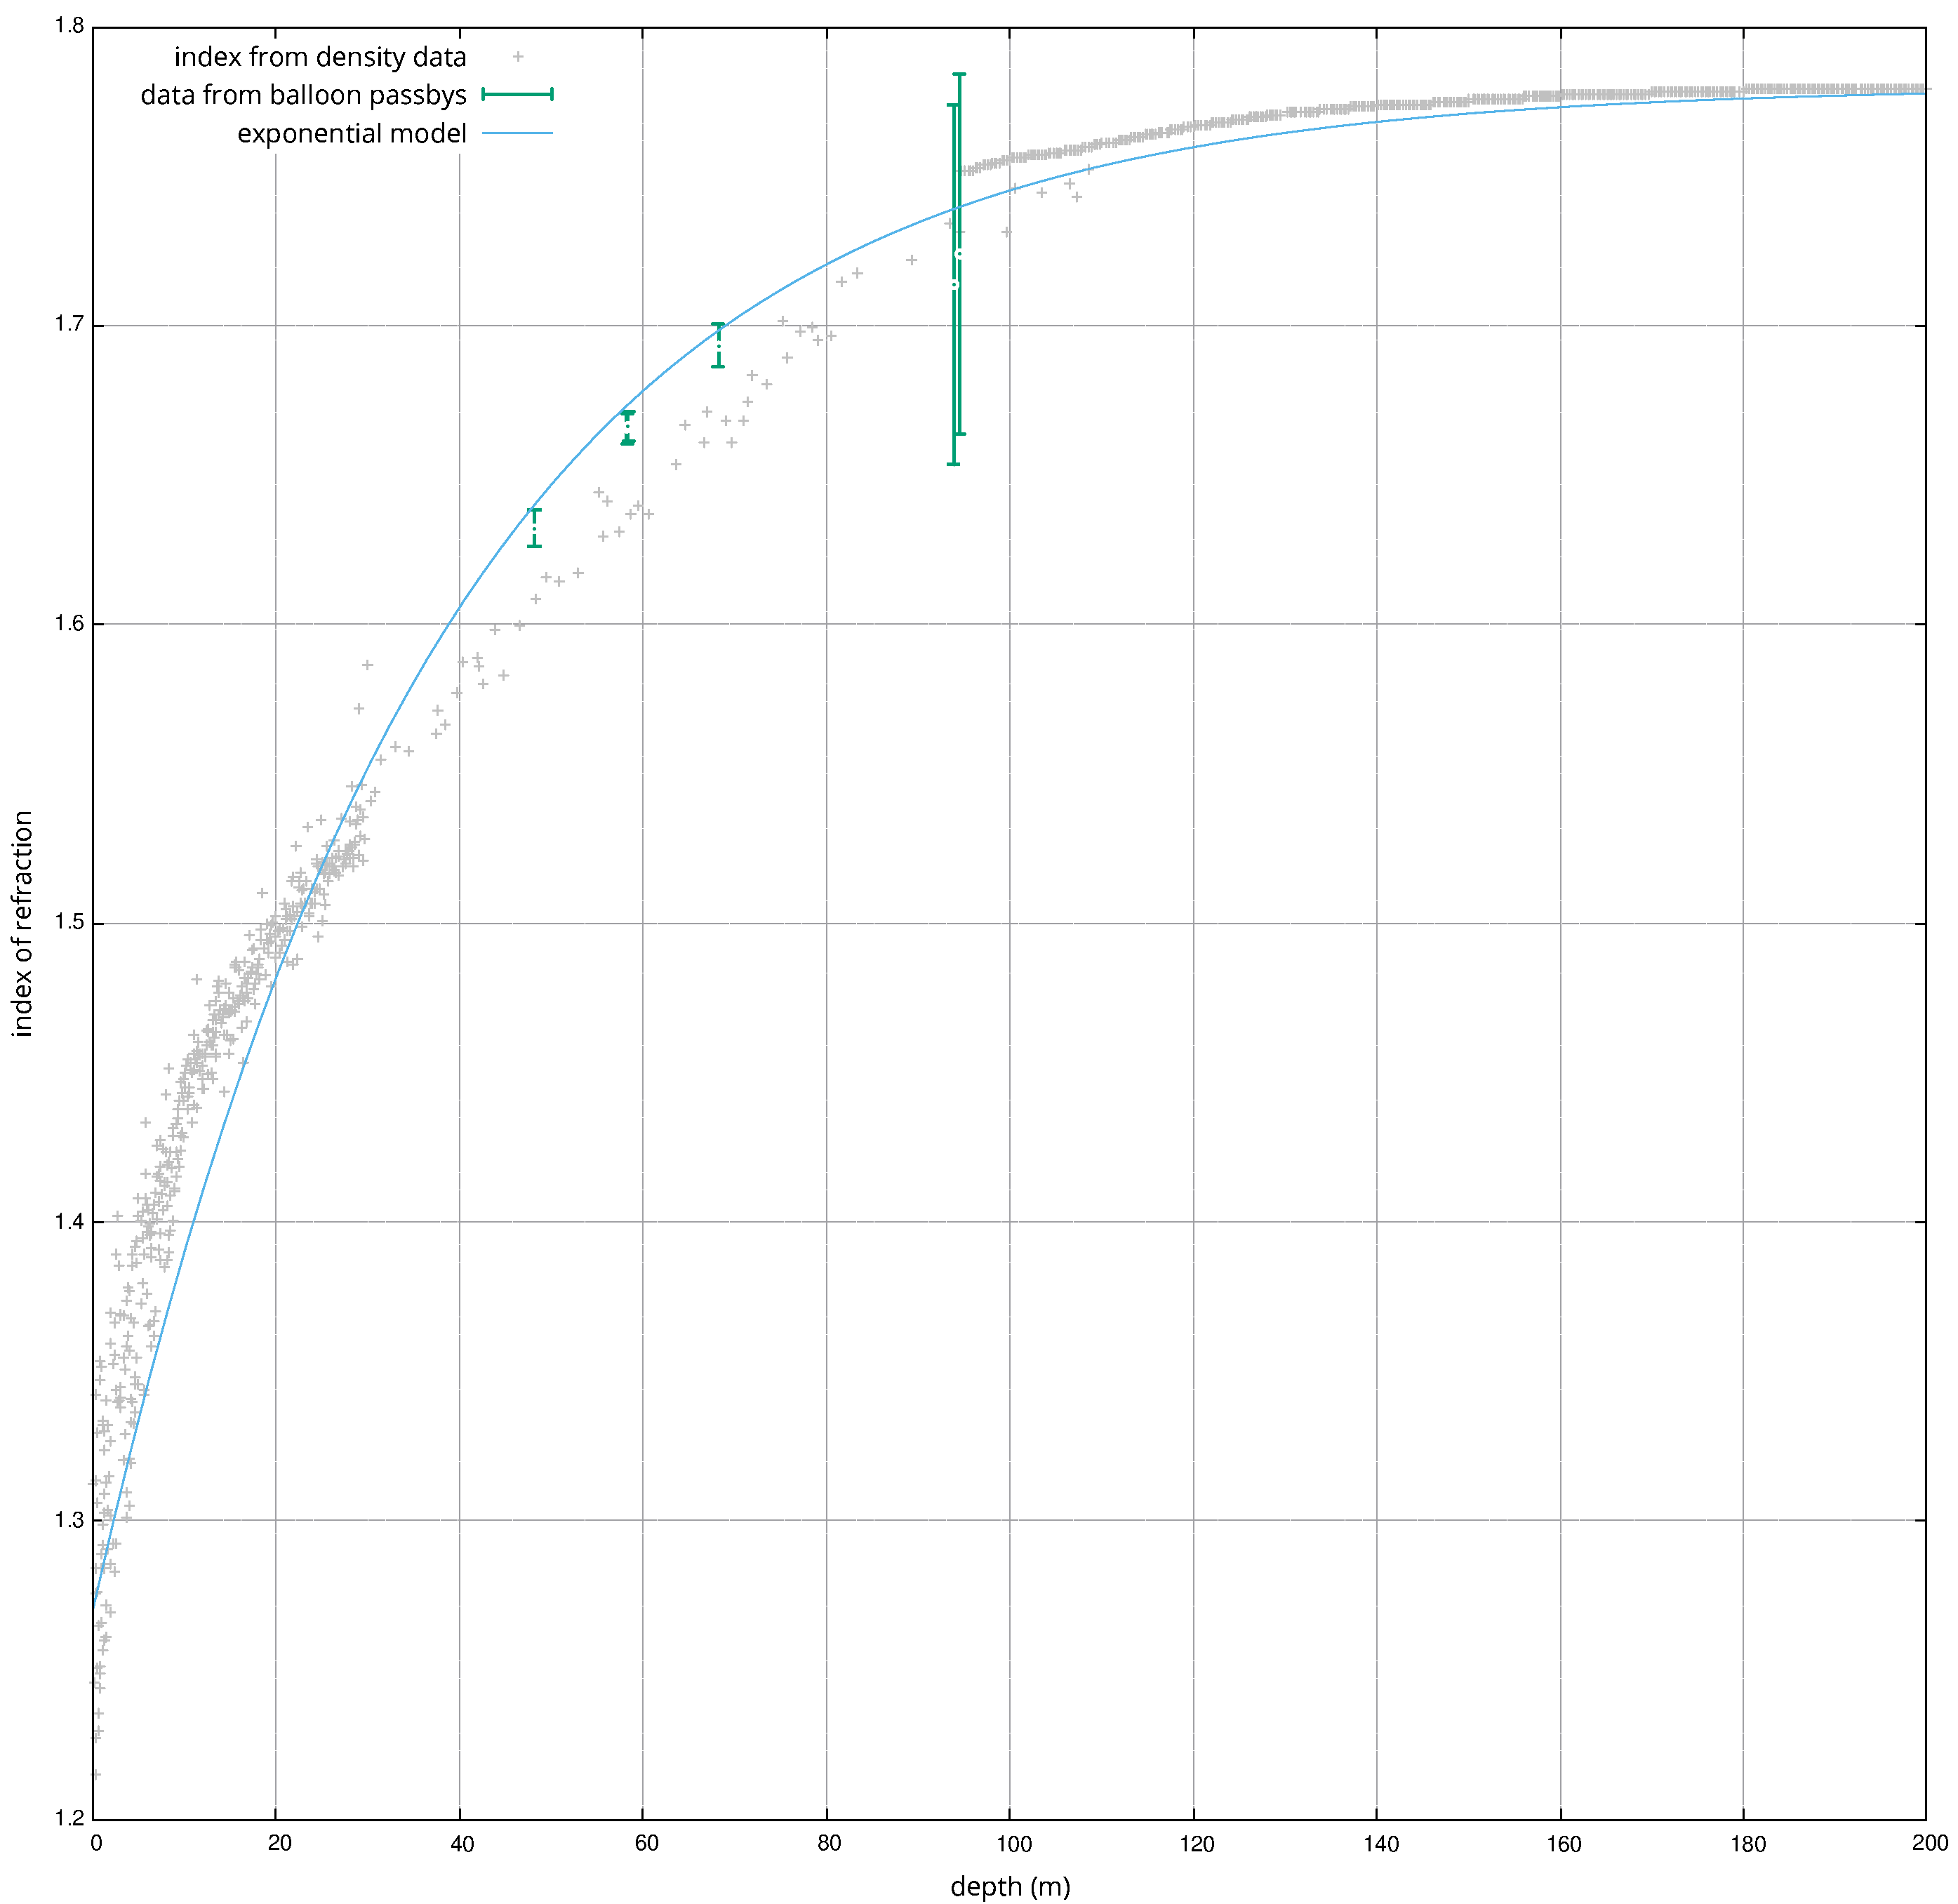
\includegraphics[width=\textwidth]{figures/ResultsBig.pdf}
  \caption{In this bigger plot it's easier to see just where our measured values lie.}
	\label{fig:ResultsBig}
\end{figure}
\chapter{Balloon passbys under 5°\\ in the summer of 2022}
\label{app:5Deg}
\csvautotabular{tables/EventsBelow5DegPart1.csv}
\csvautotabular{tables/EventsBelow5DegPart2.csv}
\csvautotabular{tables/EventsBelow5DegPart3.csv}
\chapter{Balloon passbys under 10°\\ in the summer of 2022}
\label{app:10Deg}
\begin{table}[h!]
\csvautotabular{tables/EventsBelow10DegPart5.csv}
\end{table}
\begin{table}
\csvautotabular{tables/EventsBelow10DegPart1.csv}
\end{table}
\begin{table}
\csvautotabular{tables/EventsBelow10DegPart2.csv}
\end{table}
\begin{table}
\csvautotabular{tables/EventsBelow10DegPart3.csv}
\end{table}
\begin{table}
\csvautotabular{tables/EventsBelow10DegPart4.csv}
\end{table}
